% OpenMP для разных стратегий распараллеливания для Римановского решателя.
\subsection{Исследование масштаибруемости плотных параллельных вычислений на микропроцессорах Intel}

\begin{figure}[ht]
	\centering
	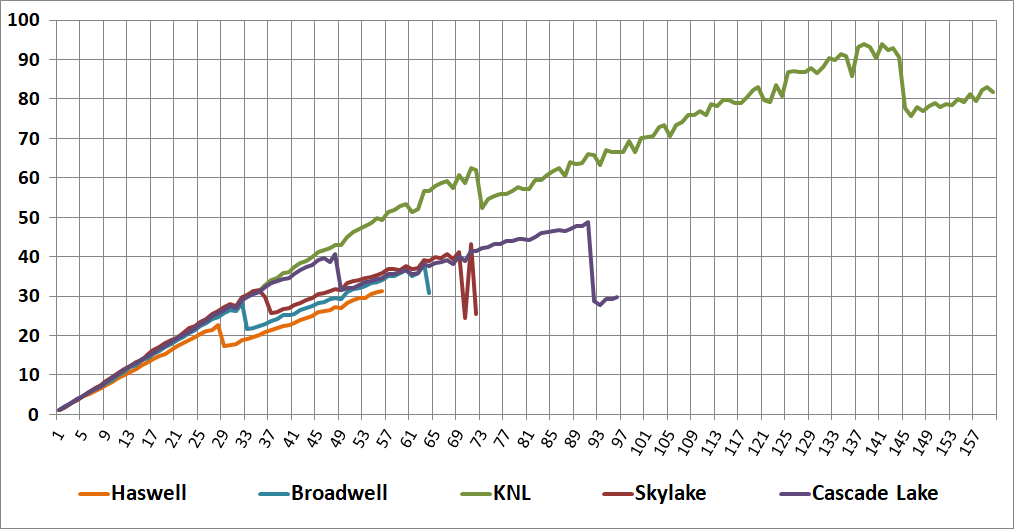
\includegraphics[width=1.0\textwidth]{./pics/text_3_omp2/speedup_scalar.png}
	\caption{График ускорения скалярной версии римановского решателя для микропроцессоров Haswell, Broadwell, KNL, Skylake, Cascade Lake для количества потоков от 1 до 160.}
	\label{fig:text_3_omp2_speedup_scalar}
\end{figure}

\begin{figure}[ht]
	\centering
	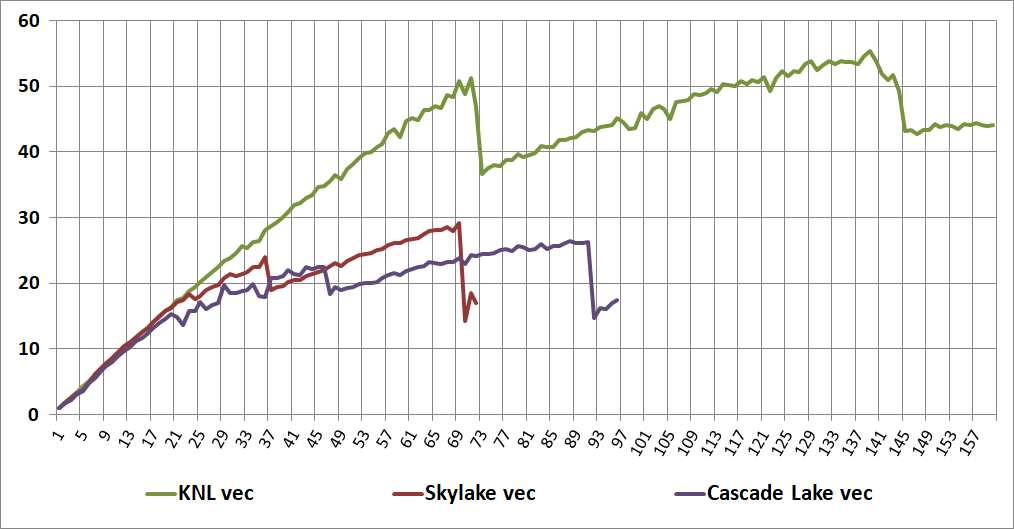
\includegraphics[width=1.0\textwidth]{./pics/text_3_omp2/speedup_vec.png}
	\caption{График ускорения векторизованной версии римановского решателя для микропроцессоров KNL, Skylake, Cascade Lake для количества потоков от 1 до 160.}
	\label{fig:text_3_omp2_speedup_vec}
\end{figure}

\begin{figure}[ht]
	\centering
	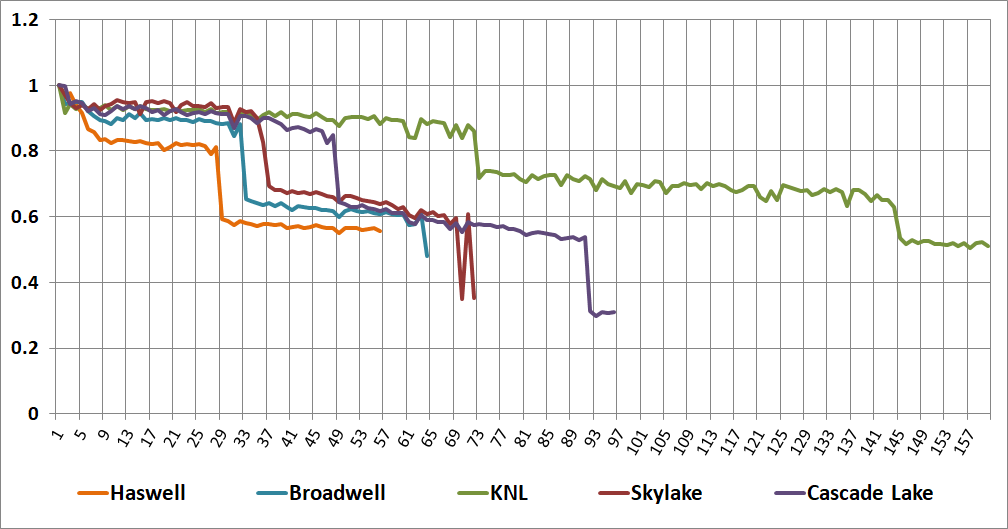
\includegraphics[width=1.0\textwidth]{./pics/text_3_omp2/eff_scalar.png}
	\caption{График масштабируемости скалярной версии римановского решателя для микропроцессоров Haswell, Broadwell, KNL, Skylake, Cascade Lake для количества потоков от 1 до 160.}
	\label{fig:text_3_omp2_eff_scalar}
\end{figure}

\begin{figure}[ht]
	\centering
	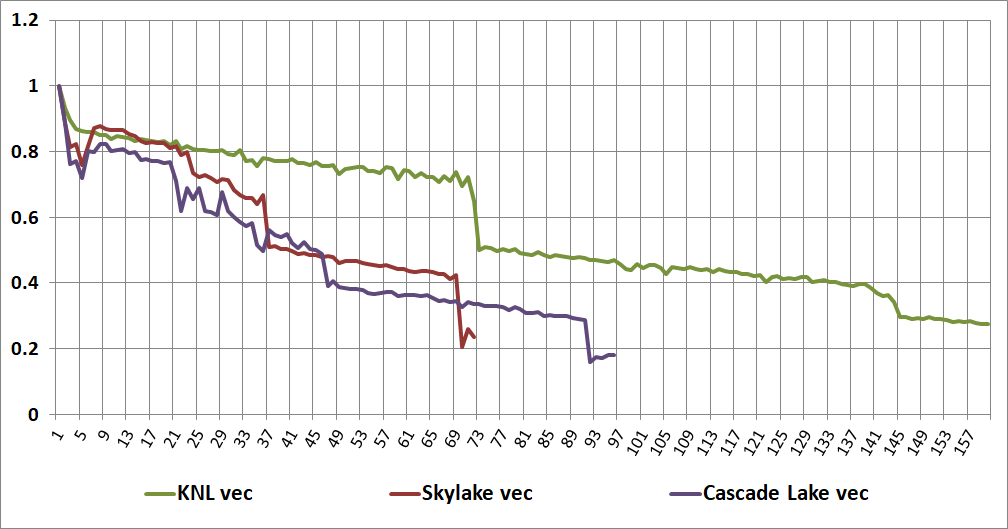
\includegraphics[width=1.0\textwidth]{./pics/text_3_omp2/eff_vec}
	\caption{График масштабируемости векторизованной версии римановского решателя для микропроцессоров KNL, Skylake, Cascade Lake для количества потоков от 1 до 160.}
	\label{fig:text_3_omp2_eff_scalar}
\end{figure}
